\documentclass{beamer}

\mode<presentation>
{
  \usetheme{Frankfurt}
  \usecolortheme{orchid}
  \setbeamercovered{invisible}
  \setbeamertemplate{footline}[frame number]
}

\usepackage[english]{babel}
\usepackage[latin1]{inputenc}
\usepackage{times}
\usepackage[T1]{fontenc}
\usepackage{tikz}
\usepackage{array}
\usepackage{cancel}


\usetikzlibrary{shapes,backgrounds}

\def\multiset#1#2{\ensuremath{\left(\kern-.3em\left(\genfrac{}{}{0pt}{}{#1}{#2}\right)\kern-.3em\right)}}

\def\blue{\color{blue}~}
\def\black{\color{black}~}
\def\bl[#1]#2{\begin{block}{#1}#2\end{block}}
\def\integers{\mathbb{Z}}
\def\enumb{\begin{enumerate}}
\def\enume{\end{enumerate}}
\def\itemb{\begin{itemize}}
\def\iteme{\end{itemize}}


\usepackage{remreset}
\makeatletter
\@removefromreset{subsection}{section}
\makeatother
\setcounter{subsection}{1}

\title{Discrete Mathematics, Section 001, Fall 2016}
\subtitle{Lecture 16: Composition of functions, Operations, Symmetries}
\date{November 7, 2016}

\author[Zsolt]{Zsolt Pajor-Gyulai \\ \texttt{zsolt@cims.nyu.edu}}

\pgfdeclareimage[height=1cm]{NYUlogo}{NYUlogo.jpg}

\institute[NYU] 
{
\normalsize Courant Institute of Mathematical Sciences
}
\titlegraphic{\pgfuseimage{NYUlogo}}

\begin{document}

\begin{frame}
  \titlepage
\end{frame}

\AtBeginSection[]
{
\begin{frame}
\frametitle{Outline}
\tableofcontents[currentsection]
\end{frame}}

\section{Composition}

\begin{frame}{The natural operation to combining functions}
\bl[Definition]{Let $A,B$, and $C$ be sets and let $f:A\to B$ and $g:B\to C$. Then $g\circ f:A\to C$ is defined by
\[
(g\circ f)(a)=g[f(a)],\qquad a\in A.
\]
The function $g\circ f$ is called \textbf{the composition} of $g$ and $f$.}
For example, let 
\[
A=\{1,2,3,4,5\}\qquad B=\{6,7,8,9\}\qquad C=\{10,11,12,13,14\}.
\]
Let \vspace{-0.3cm}
\[
f=\{(1,6),(2,6),(3,9),(4,7),(5,7)\}
\]
\[
g=\{(6,10),(7,11),(8,12),(9,13)\}.
\]\vspace{-0.2cm}
Then\vspace{-0.2cm}
\[
(g\circ f)=\{(1,10),(2,10),(3,13),(4,11),(5,11)\}.
\]
\end{frame}

\begin{frame}
\bl[Further example]{
Let $f:\mathbb{Z}\to\mathbb{Z}$ and $g:\mathbb{Z}\to\mathbb{Z}$ defined by
\[
f(x)=x^2+1,\qquad g(x)=2x-3
\]
Then
\begin{align*}
(g\circ f)(x)&=g[f(x)]=g(x^2+1)=\\
&=2(x^2+1)-3=2x^2+2-3=2x^2-1.
\end{align*}}

Remarks:
\itemb
\item Note the order in $(g\circ f)(a)$. $f$ is closer and hits $a$ first.
\item $\textrm{Dom}(g\circ f)=\textrm{Dom}f$.
\[
f:A\to B,\qquad g:B\to C\qquad \to\qquad\textrm{Im}f\subseteq B=\textrm{Dom}g
\]
\iteme

\end{frame}

\begin{frame}
\bl[]{\textbf{Q}: Is $f\circ g=g\circ f$?}
\itemb
\item This only makes sense in the first place if $f:A\to A$ and $g:A\to A$.
\item Even then, this is not true in general!
\iteme
For example, let $A=\{1,2,3,4,5,6\}$ and $f:A\to A$, $g:A\to A$ defined by
\[
f=\{(1,1),(2,1),(3,1),(4,1),(5,1)\},
\]
\[
g=\{(1,5),(2,4),(3,3),(4,2),(5,1)\}.
\]
Then
\[
g\circ f=\{(1,5),(2,5),(3,5),(4,5),(5,5)\},
\]
\[
f\circ g=\{(1,1),(2,1),(3,1),(4,1),(5,1)\}.
\]
Thus
\bl[]{\[
g\circ f\neq f\circ g
\]}
\end{frame}

\begin{frame}
Another example, $f,g:\mathbb{Z}\to\mathbb{Z}$
\[
f(x)=x^2+1,\qquad g(x)=2x-3
\]
Then
\begin{align*}
(g\circ f)(x)=g[f(x)]=g[x^2+1]=2(x^2+1)-3=2x^2-1
\end{align*}
\begin{align*}
(f\circ g)(x)=f[g(x)]=f[2x-3]=(2x-3)^2+1=4x^2-12x+10
\end{align*}
Once again 
\bl[]{\[
g\circ f\neq f\circ g
\]}
\center\color{red}Composition is not commutative!\color{black}

\begin{center}{Do Problem 1 on the WS!}\end{center}
\end{frame}

\begin{frame}
What about associativity?
\bl[Proposition]{Let $A$,$B$,$C$, and $D$ be sets and let $f:A\to B$, $g:B\to C$, and $h:C\to D$. Then
\[
h\circ(g\circ f)=(h\circ g)\circ f
\]}
To prove this we need to prove the equality of functions.
\bl[Proving two functions are equal]{
Let $f$ and $g$ be functions. To prove $f=g$, do the following:
\itemb
\item Prove that $\textrm{Dom}f=\textrm{Dom}g$.
\item Prove that for all $x$ in the common domain, $f(x)=g(x)$.
\iteme}
\end{frame}

\begin{frame}
\bl[Proposition]{Let $A$,$B$,$C$, and $D$ be sets and let $f:A\to B$, $g:B\to C$, and $h:C\to D$. Then\vspace{-0.3cm}
\[
h\circ(g\circ f)=(h\circ g)\circ f
\]}
\begin{proof}
We first check that the domains are the same.\vspace{-0.3cm}
\[
\textrm{Dom}[h\circ(g\circ f)]=\textrm{Dom}(g\circ f)=\textrm{Dom}f=A
\]\vspace{-1cm}

\[
\textrm{Dom}[(h\circ g)\circ f]=\textrm{Dom}f=A
\]
~~~~Then we check that they have the same values. For $a\in A$,
\[
[h\circ(g\circ f)](a)=h[(g\circ f)(a)]=h[g(f(a))]
\]
\[
[(h\circ g)\circ f](a)=(h\circ g)[f(a)]=h[g(f(a))]
\]
This finishes the proof of the proposition.
\end{proof}
\end{frame}

\begin{frame}{Identity function}
\bl[Definition]{Let $A$ be a set. The \textbf{identity function} on $A$ is the function $\textrm{id}_A:A\to A$, defined by $\textrm{id}_A(a)=a$. In other words,
\[
\textrm{id}_A=\{(a,a):a\in A\}.
\]}
If composition is the analogue of a product, then $\textrm{id}_A$ is the analogue of `one`.
\bl[Proposition]{Let $A$ and $B$ be sets. Let $f:A\to B$. Then
\[
f\circ\textrm{id}_A=\textrm{id}_B\circ f=f
\]}
\end{frame}

\begin{frame}{Identity function}
\bl[Proposition]{Let $A$ and $B$ be sets. Let $f:A\to B$. Then\vspace{-0.2cm}
\[
f\circ\textrm{id}_A=\textrm{id}_B\circ f=f
\]}
\begin{proof}
We first show they have the same domain: \vspace{-0.2cm}
\[
\textrm{Dom}(f\circ\textrm{id}_A)=\textrm{Dom}(\textrm{id}_A)=A
\]\vspace{-1.2cm}


\[
\textrm{Dom}(\textrm{id}_B\circ f)=\textrm{Dom}f=A
\]\vspace{-0.6cm}

Second, observe\vspace{-0.2cm}
\[
(f\circ\textrm{id}_A)(a)=f(\textrm{id}_A(a))=f(a),
\]\vspace{-0.6cm}

and $(\textrm{id}_B\circ f)(a)=f(a)$ similarly and the claim is proved.
\end{proof}

\begin{center}{Do Problem 2 on the WS!}\end{center}
\end{frame}

\section{Operations}

\begin{frame}{General notion of an operation}
Abstract algebra is the study of structures and operations.
\bl[Definition]{Let $A$ be a set. A \textbf{binary operation} on $A$ is a function whose domain is $A\times A$.}
For example,
\itemb
\item $+:\mathbb{R}\times\mathbb{R}\to\mathbb{R}$, $+(a,b)=a+b$.
\item $f:\mathbb{Z}\times\mathbb{Z}\to\mathbb{Z}$, $f(x,y)=|x-y|$
\iteme
Commonly used symbol for operations: $*$

Notation: $*(a,b)=a*b$.\vspace{0.5cm}

When we want to emphasize what the set $A$ is, we use the notation $(A,*)$. The two above examples then are
\[
(\mathbb{R},+),\qquad (\mathbb{Z},f)
\]
\end{frame}

\begin{frame}{Other examples}
\itemb
\item $+$ is an operation on $\mathbb{N}$ and $a+b\in \mathbb{N}$ whenever $a,b\in \mathbb{N}$. (\textbf{closure property})
\item $-$ is an operation on $\mathbb{N}$ but $a-b$ might not be a natural for every $a,b\in\mathbb{N}$.
\item $\cdot$ is an operation on $\mathbb{N}$ and the closure property holds.
\item $/$ is not an operation on $\mathbb{N}$ as e.g. $(2,0)$ is not in its domain.
\item $/$ is, however, a relation on the positive integers.
\item $\circ$ is an operation on the set of functions from $A^A$ (set of functions from $A$ to $A$).
\iteme

This week, we are going to learn about another interesting examples: permutations.
\end{frame}

\begin{frame}{Properties of operations}
\bl[Commutative property]{Let $*$ be an operation on a set $A$. We say that * is \textbf{commutative} on $A$ provided
\[
\forall a,b\in A, a*b=b*a
\]}
For example, 
\itemb
\item $+$ is commutative on $\mathbb{Z}$
\item $\circ$ is not commutative on $A^A$. 
\item $-$ is not commutative on $\mathbb{Z}$.
\iteme
\end{frame}

\begin{frame}{Properties of operations}
\bl[Closure property]{Let $*$ be an operation on a set $A$. We say that $*$ is closed on $A$ provided
\[
\forall a,b\in A, a*b\in A
\]}
For example,
\itemb
\item $\cdot$ is closed on $\mathbb{N}$
\item $-$ is not closed on $\mathbb{N}$
\item $-$ is closed on $\mathbb{Z}$.
\iteme
\end{frame}

\begin{frame}{Properties of operations}
\bl[Associative property]{Let $*$ be an operation on a set $A$. We say that $*$ is \textbf{associative} on $A$ provided
\[
\forall a,b,c\in A, (a*b)*c=a*(b*c).
\]}
For example, 
\itemb
\item $+$ and $\cdot$ are associative on $\mathbb{Z}$
\item  $-$ is not as e.g.
\[
(3-4)-7=-8\neq 6= 3-(4-7)
\]
\iteme
\end{frame}

\begin{frame}[t]{Properties of operations}

\bl[Identity element]{Let $*$ be an operation on a set $A$. An element $e\in A$ is called an \textbf{identity} for $*$ provided
\[
\forall a\in A, a*e=e*a=a
\]}
\only<1>{For example, 
\itemb
\item $0$ is an identity element for $+$ on $\mathbb{Z}$
\item $1$ is an identity element for $\cdot$ on $\mathbb{Z}$.
\item $-$ does not have an identity element on $\mathbb{Z}$ as
\[
a-0=a,\qquad\textrm{but}\qquad 0-a=-a\neq a
\]
\iteme}
\only<2>{
\bl[Proposition]{Let $*$ be an operation defined on a set $A$. Then $*$ can have at most one identity elements.}
FTSC, suppose there are two identities $e$ and $e'$ in $A$ with $e\neq e'$.
\itemb
\item On one hand $e*e'=e$ as $e'$ is an identity.
\item On the other hand $e*e'=e'$ as $e$ is an identity.
\iteme
Therefore $e=e'$ contradicting $e\neq e'$. $\Rightarrow\Leftarrow$\qed
}
\end{frame}

\begin{frame}{Properties of operations}
\bl[Inverses]{Let $*$ be an operation on a set $A$ and suppose $A$ has an identity $e$. For an element $a\in A$, we call an element $b\in A$ an \textbf{inverse} of $a$ provided $a*b=b*a=e$.}
For example,
\itemb
\item In $(\mathbb{Z},+)$, the inverse of $a\in\mathbb{Z}$ is $(-a)$.
\item In $(\mathbb{Q},\cdot)$, the inverse of $x\in\mathbb{Q}$ is $\frac{1}{x}$ when $x\neq 0$. However $x=0$ does not have an inverse!
\item Consider the following relation on $\{e,a,b,c\}$:
\begin{columns}
\column{0.4\textwidth}
\center
\begin{tabular}{|c|cccc|}
\hline
*&e&a&b&c\\
\hline
e&e&a&b&c\\
a&a&a&e&e\\
b&b&e&b&e\\
c&c&e&e&c\\
\hline
\end{tabular}
\column{0.6\textwidth}

Both $b$ and $c$ are inverses of $a$:\vspace{-0.2cm}
\[
a*b=b*a=e,\qquad a*c=c*a=e
\]\vspace{-0.6cm}\\
The inverse might not be unique.

\begin{center}{Do Problem 3 on the WS!}\end{center}
\end{columns}
\iteme
\end{frame}




\section{Symmetries}

\begin{frame}{Symmetries of the square}
\bl[Intuitively]{A \textbf{symmetry} of a figure is a motion that, when applied to an object, results in a figure that looks exactly the same as the original}
\itemb
\item Rotating a square counterclockwise about its center through an angle of $90^{\textdegree}$ is a symmetry.
\begin{figure}
\centering
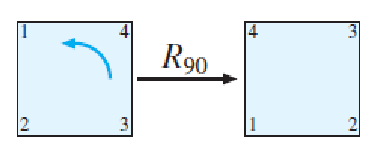
\includegraphics[scale=1]{R90.pdf}
\end{figure}
\item However, rotating by $30\textdegree$, denoted by $R_{30}$ is not a symmetry.
\iteme
\end{frame}

\begin{frame}{Symmetries of the square}
\itemb
\item In the same vein, $R_{180}$, $R_{270}$, and $R_{360}$ are also symmetries. E.g.:
\begin{figure}
\centering
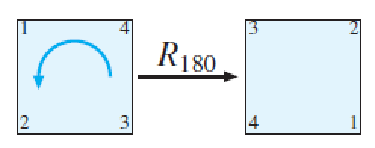
\includegraphics[scale=1]{R180.pdf}
\end{figure}
\item However, we would rather like to say that $R_{360}$ does not do anything, and we are going to call it $I$ for identity.
\iteme
With this, we have the following symmetries:
\begin{figure}
\centering
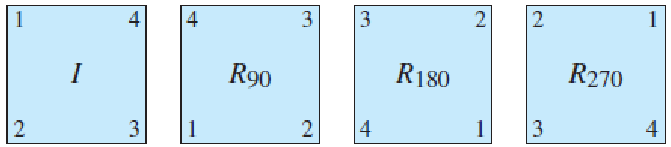
\includegraphics[scale=0.8]{Rotations.pdf}
\end{figure}

\end{frame}

\begin{frame}{Symmetries of the square}
With this, we have the following symmetries:
\begin{figure}
\centering
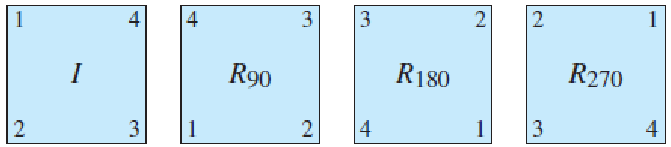
\includegraphics[scale=0.8]{Rotations.pdf}
\end{figure}
However, we have more symmetries: reflections.
\itemb
\item For example, reflection through the horizontal axis and the $SW-NE$ diagonal:

\iteme
\begin{figure}
\centering
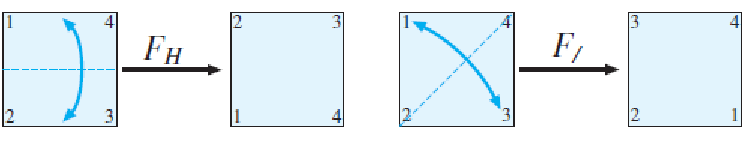
\includegraphics[scale=0.8]{FIFH.pdf}
\end{figure}
\itemb
\item Of course we have to more axis to reflect about: $-,\backslash$
\iteme
\end{frame}

\begin{frame}{Symmetries of the square}
\begin{figure}
\centering
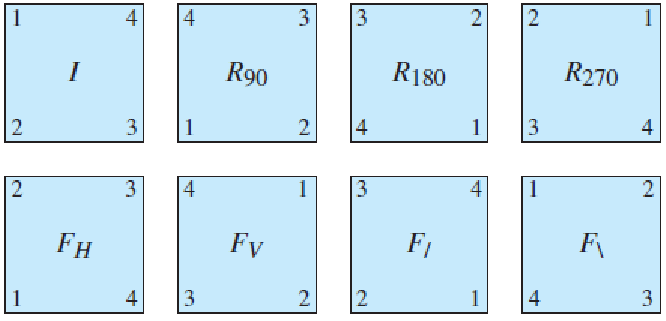
\includegraphics[scale=0.8]{Allsymm.pdf}
\end{figure}
\itemb
\item \textbf{Have we repeated ourselves?} No, notice that no two corner label arrangements are the same.
\item \textbf{Did we find all symmetries?} Yes, we exhausted all possible $2\cdot 4=8$ label arrangements. (Label $1$ can go to four places, after which for label $2$, we have two choices, after which $3,4$ are fixed.)
\iteme
\end{frame}

\begin{frame}{Combining symmetries}
Applying symmetries consecutively, the result will also be a symmetry. For example,
\begin{figure}
\centering
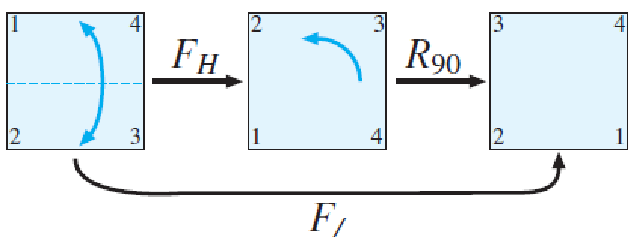
\includegraphics[scale=0.8]{R90circFH.pdf}
\end{figure}
Since the result is a symmetry it must be one of the $8$ ones that we have listed!
\[
R_{90}\circ F_H=F_I
\]
where the left hand side means applying $F_H$ first and then $R_{90}$.
\end{frame}

\begin{frame}{`Multiplication table for the symmetries of squares'}
If we figure out all the combinations:
\begin{figure}
\centering
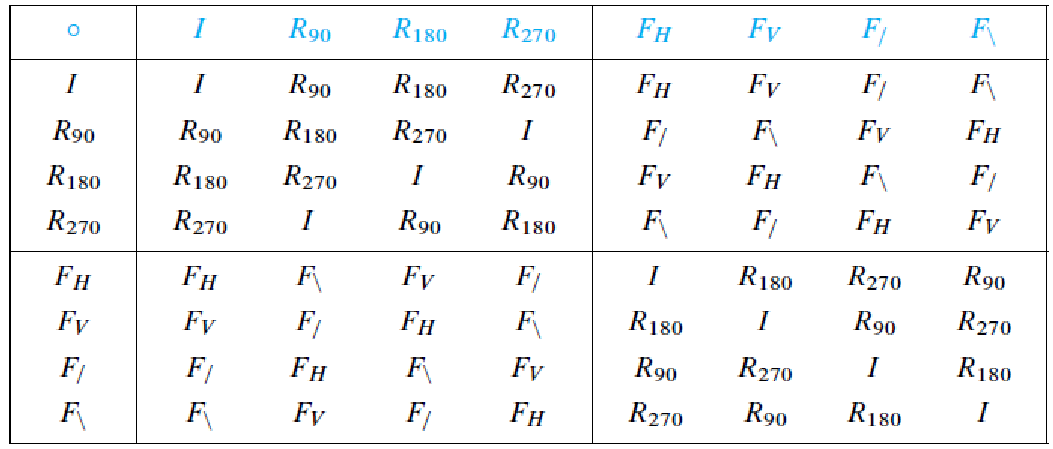
\includegraphics[scale=0.6]{Multipltable.pdf}
\end{figure}
\itemb
\item Note that, $R_{90}\circ F_H=F_{/}\neq F_{\backslash}=F_H\circ R_{90}$, and therefore $\circ$ is not commutative.
\item $I$ is the identity element for $\circ$.
\item Every element has an inverse.
\iteme
\end{frame}

\begin{frame}{Symmetries as permutations}
\begin{figure}
\centering
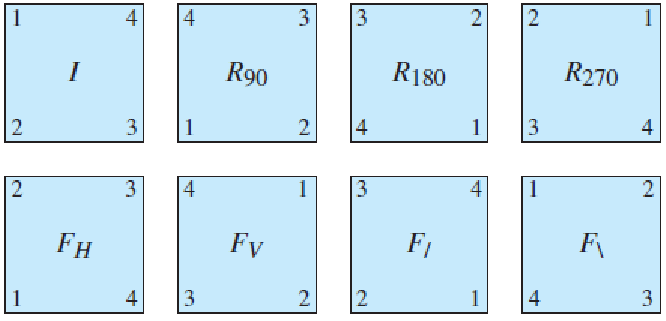
\includegraphics[scale=0.8]{Allsymm.pdf}
\end{figure}\vspace{-0.2cm}
\itemb
\item Note that if I tell you where the labels $1,2,3,4$ go, you can identify the symmetry! 
\item For example, $R_{90}$ can be represented as a function 
\[
R_{90}:\{1,2,3,4\}\to\{1,2,3,4\}
\]
\[
R_{90}(1)=2,\qquad R_{90}(2)=3,\qquad R_{90}(3)=4,\qquad  R_{90}(4)=1
\]
\iteme

\end{frame}

\begin{frame}{Symmetries as permutations}
\begin{figure}
\centering
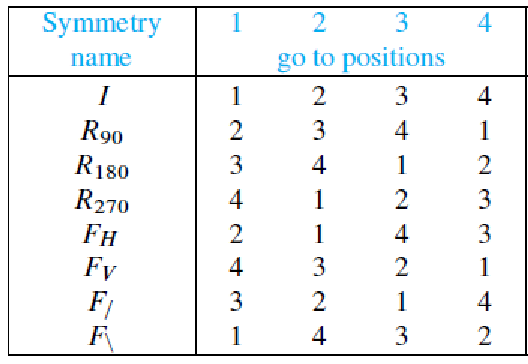
\includegraphics[scale=0.8]{Asperm.pdf}
\end{figure}
Convenient notation:
\[
R_{90}=\left[\begin{array}{cccc}
1&2&3&4\\
2&3&4&1
\end{array}\right]\qquad F_H=\left[\begin{array}{cccc}
1&2&3&4\\
2&1&4&3
\end{array}\right]
\]
\end{frame}
\end{document}